\documentclass[a4paper,10pt]{amsbook}

\usepackage[T1]{fontenc}
\usepackage{lmodern}
\usepackage[utf8x]{inputenc}
\usepackage[italian]{babel}

\usepackage{amsmath}
\usepackage{amssymb}
\usepackage{amsthm}
\usepackage{xfrac}
\usepackage[all]{xy}
\usepackage{graphicx}
\usepackage{algorithm}
\usepackage[noend]{algpseudocode}
%\usepackage{fullpage}
\usepackage{hyperref}



%\setlength{\parindent}{0in}

\newcounter{counter1}

\theoremstyle{plain}
\newtheorem{myteo}[counter1]{Teorema}
\newtheorem{mylem}[counter1]{Lemma}
\newtheorem{mypro}[counter1]{Proposizione}
\newtheorem{mycor}[counter1]{Corollario}
\newtheorem*{myteo*}{Teorema}
\newtheorem*{mylem*}{Lemma}
\newtheorem*{mypro*}{Proposizione}
\newtheorem*{mycor*}{Corollario}

\theoremstyle{definition}
\newtheorem{mydef}[counter1]{Definizione}
\newtheorem{myes}[counter1]{Esempio}
\newtheorem{myex}[counter1]{Esercizio}
\newtheorem*{mydef*}{Definizione}
\newtheorem*{myes*}{Esempio}
\newtheorem*{myex*}{Esercizio}

\theoremstyle{remark}
\newtheorem{mynot}[counter1]{Nota}
\newtheorem{myoss}[counter1]{Osservazione}
\newtheorem*{mynot*}{Nota}
\newtheorem*{myoss*}{Osservazione}


\newcommand{\obar}[1]{\overline{#1}}
\newcommand{\ubar}[1]{\underline{#1}}

\newcommand{\set}[1]{\left\{#1\right\}}
\newcommand{\pa}[1]{\left(#1\right)}
\newcommand{\ang}[1]{\left<#1\right>}
\newcommand{\bra}[1]{\left[#1\right]}
\newcommand{\abs}[1]{\left|#1\right|}
\newcommand{\norm}[1]{\left\|#1\right\|}
\newcommand{\ceil}[1]{\left\lceil#1\right\rceil}
\newcommand{\floor}[1]{\left\lfloor#1\right\rfloor}

\newcommand{\pfrac}[2]{\pa{\frac{#1}{#2}}}
\newcommand{\bfrac}[2]{\bra{\frac{#1}{#2}}}
\newcommand{\psfrac}[2]{\pa{\sfrac{#1}{#2}}}
\newcommand{\bsfrac}[2]{\bra{\sfrac{#1}{#2}}}

\newcommand{\der}[2]{\frac{\partial #1}{\partial #2}}
\newcommand{\pder}[2]{\pfrac{\partial #1}{\partial #2}}
\newcommand{\sder}[2]{\sfrac{\partial #1}{\partial #2}}
\newcommand{\psder}[2]{\psfrac{\partial #1}{\partial #2}}

\newcommand{\intl}{\int \limits}

\DeclareMathOperator{\de}{d}
\DeclareMathOperator{\id}{Id}
\DeclareMathOperator{\len}{len}

\DeclareMathOperator{\gl}{GL}
\DeclareMathOperator{\aff}{Aff}
\DeclareMathOperator{\isom}{Isom}

\DeclareMathOperator{\im}{Im}

\makeatletter
\@beginparpenalty=10
\makeatother

\title{Tesi}
\author{Enrico Polesel}
\date{\today}

\begin{document}
\maketitle

\setcounter{tocdepth}{5}



\tableofcontents

\chapter{Cammini minimi su grafi}

\begin{mydef}[Grafo]
  Chiamiamo grafo la coppia $G = (V,E)$ dove $V$ è un insieme finito
  di elementi detti \textit{nodi} e $E\subseteq V \times V$ di
  relazioni chiamate archi.
\end{mydef}

Se non specificato diversamente definiamo $N = \abs{V}$ e $M =
\abs{E}$.

Diciamo che gli archi di un grafo sono pesati se esiste una funzione
\textit{peso}
\[ w : E \rightarrow \mathbb{R} \]
Per noi il peso di un arco rappresenta la sua lunghezza, per questo
chiameremo \textit{lunghezza di un arco} il suo peso.

Nel caso non pesato ci riconduciamo al caso pesato prendendo $w$
costante a $1$.

Siamo interessati a considerare grafi diretti, cioè gli archi sono
orientati, nel caso indiretto possiamo ridurci a questo caso
considerando l'insieme di archi 
\[ V' = V \cup \set{ (v,u) \mid (u,v) \in V } \]

\section{Proprietà dei cammini minimi}

\begin{mydef}[Cammino]
  Chiamiamo \textit{cammino} sul grafo $G$ una successione ordinata
  finita di nodi $p = ( v_0, v_1, ..., v_k)$ tale che 
  \[ \forall i \in \set{ 1, ... , k} \;\;\; (v_{i-1}, v_{i} ) \in E\]
\end{mydef}

Diciamo che $p$ congiunge $v_0$ a $v_k$. Dati due nodi $v,w$ chiamiamo
$P(u,v)$ l'insieme (eventualmente vuoto) dei cammini che congiungono
$u$ a $v$

Dati due cammini $p = ( v_0, v_1, ..., v_k)$ e $q = ( u_0, u_1, ...,
u_{h})$ tali che $v_k = u_0$ chiamiamo somma dei due cammini il
cammino
\[ p+q = ( v_0, v_1, ..., v_k= u_0, u_1, ..., u_{h}) \]

Dato un cammino $p = ( v_0, v_1, ..., v_k)$ chiamiamo
\textit{sottocammino} di $p$ un cammino $q = ( v_i , v_{i+1}, ... ,
v_j )$ con $0 \le i \le j \le k$.

\begin{mydef}[Lunghezza di un cammino]
  Chiamiamo lunghezza di un cammino $p$ la quantità
  \[ w(p) = \sum _{i=1} ^k w \pa{ (v_{i-1}, v_i) } \]
\end{mydef}

Osserivamo che la lunghezza della somma di due cammini è uguale alla
somma delle lunghezze.

Siamo interessati a trattare grafi in cui gli archi hanno lunghezza
non negativa, per cui da ora usiamo l'ipotesi $\forall e \in E \; w(e)
\ge 0$.

\begin{mydef}[Distanza di due punti]
  \[ \delta(u,v) = \left\{
    \begin{matrix}
      \min \limits_{p \in P(u,v)} { w(p) } & \; P(u,v) \neq \emptyset \\
      \infty & \; P(u,v) = \emptyset
    \end{matrix}
    \right.
    \]
\end{mydef}

Per $P(u,v) \neq \emptyset$ chiamiamo \textit{cammino minimo} fra $u$
e $v$ un cammino la cui lunghezza realizza il minimo.

Osserviamo che questa distanza verifica le proprietà
\begin{itemize}
\item $\delta(v,v) = 0$ infatti il cammino $(v)$ ha lunghezza $0$
\item $\delta(u,z) \le \delta(u,v) + \delta(v,z)$ infatti sommando il
  cammino minimo tra $u$ e $v$ e quello tra $v$ e $z$ si ottiene un
  cammino in $P(u,z)$
\end{itemize}
Questa distanza, però, in generale non è simmetica, quindi definisce
una pseudometrica. Nel caso di grafi non orientati allora $\delta$
diventa una distanza.

Osserviamo inoltre che
\begin{itemize}
\item Ogni sottocammino di un cammino minimo è ancora minimo
\item Possiamo sempre scegliere un cammino minimo aciclico, infatti i
  cicli contenuti in un cammino minimo devono avere lunghezza nulla
  (visto che lavoriamo in ipotesi di lunghezze non negative) e quindi
  possono essere eliminati
\end{itemize}

\section{Cammini minimi da una sorgente unica}

Fissiamo un nodo $s \in V$ che chiameremo sorgente. Siamo interessati
a calcolare:
\begin{itemize}
\item le distanze $\delta(s,v)$ al variare di $v\in V$
\item i cammini minimi tra $s$ ed ogni nodo $v\in V$
\end{itemize}

Possiamo costruire il grafo dei cammini minimi con sorgente in $s$ che
chiamiamo $G_s = (V,E_s)$ dove
\[ E_s = \set{ e\in E | e\text{ compare in un cammino minimo con
    sorgente }s} \]

Questo grafo rappresenta tutti i cammini minimi con sorgente $s$.

\begin{mypro}
  Se gli archi hanno lunghezza strettamente positiva $G_s$ definito
  come sopra è un DAG (grafo aciclico diretto)
\end{mypro}
\begin{proof}
  Supponiamo, per assurdo, che esista un ciclo $(v_0,v_1,...,v_k)$ e
  siano rispettivamente $d_0,d_1,...,d_k$ le distanze di questi nodi
  dalla sorgente $s$.

  Per ogni arco $(v_{i-1},v_i)$ abbiamo supposto che esista un cammino
  minimo che lo attraversi, troncando questo cammino otteniamo un
  cammino minimo da $s$ a $v_i$ e, troncandolo ulteriormente, un
  cammino minimo da $s$ a $v_{i-1}$. Quindi
  \[ d_k = d_{k-1} + w\pa{ (v_{i-1} , v_i ) } \Rightarrow d_i >
  d_{i-1} \]
  
  Applicando lo stesso argomento all'arco $(v_k,v_0)$ otteniamo $d_0 >
  d_k$. Unendo queste disuguaglianze otteniamo
  \[ d_0 < d_1 < \dots < d_k < d_0 \Rightarrow d_0 < d_0 \]
  Assurdo.
\end{proof}

Se invece scegliamo (in modo opportuno) un cammino minimo per ogni
nodo otteniamo un albero di cammini minimi. Per ottenere questa
struttura procediamo in modo induttivo

\textbf{Caso base:} inseriamo la sorgente $s$ nell'albero

\textbf{Passo induttivo:} scegliamo un nodo $v$ non ancora incluso
nell'albero ma raggiungibile da $s$, sia $\tilde p = (s=v_0,v_1,...,
v_{k-1}, v_k=v)$ un cammino minimo da $s$ a $v$. Prendiamo ora $h =
\max\set{ i \mid v_i \text{ appartiene all'albero}}$ e $q$ il cammino
minimo nell'albero da $s$ a $v_h$. Allora $p = q + (v_{h+1}, \dots ,
v)$ è un cammino minimo da $s$ a $v$, aggiungiamo i nodi $\pa{ v_i }
_{i>h}$ e gli archi $\pa{(v_{i-1},v_i)}_{i>h}$ all'albero.

Osserviamo che nel passo induttivo non abbiamo aggiunto nessun ciclo
all'albero, quindi il passo induttivo trasforma alberi in alberi.

Dato un albero di cammini minimi, per ogni nodo $v\in V$ definiamo:
\begin{itemize}
\item $v.d = \delta(s,v)$
\item $v.p$ il predecessore di $v$ nel cammino minimo scelto (che può
  essere indefinito nel caso in cui $v$ non sia raggiungibile da $s$
\end{itemize}

\subsection{Archi non pesati: BFS}

Nel caso in cui tutti gli archi hanno lunghezza $1$ l'albero dei
cammini minimi può essere costruito con una visita in ampiezza (BFS:
breadth-first search).

\begin{figure}[h]
  \centering
  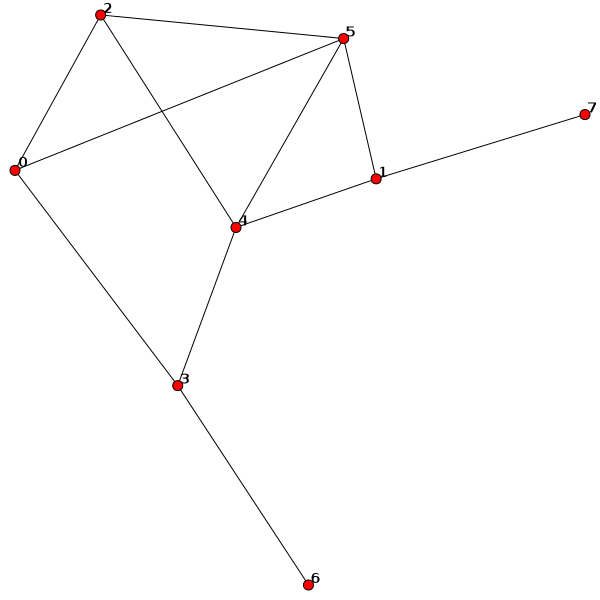
\includegraphics[width=0.9\textwidth]{preBFS}
  \caption{Esempio di un grafo indiretto non pesato}
  \label{fig:preBFS}
\end{figure}


\begin{figure}[H]
  \begin{algorithmic}
    \For {v $\in$ V} \State{v.d = $\infty$} \State{v.p = v}
    \EndFor
    \State{s.d = 0} \State{q = Queue()} \State{q.push(s)} \While{ !
      q.empty()} \State{v = q.pop()} \For{u $\in$ v.neigh} \If{u.d =
      $\infty$} \State{u.d = v.d + 1} \State{u.p = v}
    \State{q.push(u)}
    \EndIf
    \EndFor
    \EndWhile
  \end{algorithmic}
%  \caption{Pseudocodice per la BFS}
\label{fig:BFScode}
\end{figure}
Non dimostreremo che questo algoritmo è corretto; osserviamo solamente
che l'algoritmo termina in $O (M)$, infatti ogni nodo viene
inserito ed estratto dalla coda esattamente una volta e ogni arco
viene visitato una volta durante la visita del nodo di partenza.

\begin{figure}[h]
  \centering
  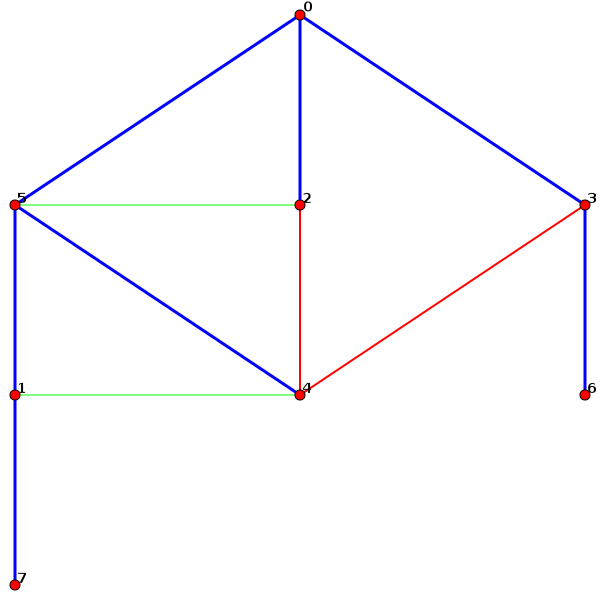
\includegraphics[width=0.9\textwidth]{BFS}
  \caption{Il grafo precedente dopo aver applicato una BFS con
    sorgente $0$, in blu gli archi scelti per l'albero, in rosso gli
    archi non scelti ma comunque appartenenti al DAG dei cammini
    minimi, in verde gli archi non appartenenti a cammini minimimi}
  \label{fig:BFS}
\end{figure}

I cammini minimi possono essere estratti in modo ricorsivo:
\begin{itemize}
\item \textbf{Caso base:} il cammino minimo da $s$ a $s$ \`e $(s)$.
\item \textbf{Passo induttivo:} un cammino minimo da $s$ a $v$ \`e
  $\tilde p + (v)$ dove $\tilde p$ \`e un cammino minimo da $s$ a $v.p$.
\end{itemize}

\subsection{Archi pesati: Dijkstra}

Nel caso in cui gli archi non abbiano tutti lunghezza unitaria, ma
comunque non negativa, dobbiamo usare l'algoritmo di Dijkstra

\begin{figure}[H]
  \begin{algorithmic}
    \For {v $\in$ V} \State{v.d = $\infty$} \State{v.p = v}
    \EndFor
    \State{S = $\emptyset$} \State{s.d = 0} \State{q =
      PriorityQueue()} \State{q.push(s,s.d)} \While{ ! q.empty()}
    \State{v = q.extract\_min()} \State{S = S $\cup$ \{v\}} \For{u
      $\in$ v.neigh} \If{u.d > v.d + w((v,u))} \State{u.d = v.d + 1}
    \State{u.p = v} \State{q.push(u,u.d)}
    \EndIf
    \EndFor
    \EndWhile
  \end{algorithmic}
%\caption{Pseudocodice per Dijkstra}
\end{figure}
Anche questa volta possiamo disegnare l'albero dei cammini minimi con
la stessa procedura usata per il caso della BFS.

Per la complessit\`a vediamo che ogni arco viene visitato esattamente
una volta e, per ogni visita, viene effettuato un inserimento nella
PriorityQueue. Il numero di estrazioni dalla PriorityQueue \`e
maggiorato dal numero di inserimenti, quindi la complessit\`a di
Dijkstra \`e $O(M\log N)$ utilizzando una coda di priorit\`a
implementata con un min-heap.

\begin{figure}[h]
  \centering
  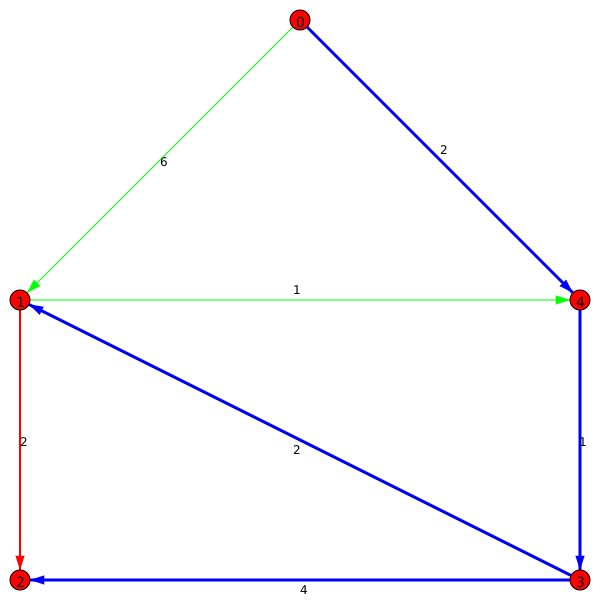
\includegraphics[width=0.9\textwidth]{dijkstra}
  \caption{Un grafo diretto pesato a cui è stato applicato Dijkstra
    con sorgente $0$, in blu gli archi scelti per l'albero, in rosso gli
    archi non scelti ma comunque appartenenti al DAG dei cammini
    minimi, in verde gli archi non appartenenti a cammini minimimi}
  \label{fig:dijkstra}
\end{figure}


\section{Cammini minimi fra ogni coppia}

Abbiamo visto che siamo in grado, data una sorgente $s\in V$, di
trovare tutti i cammini minimi da $s$ ad ogni nodo $v\in V$ e di
salvarci le distanze di ogni nodo dalla sorgente fissata. Ripetendo
questo procedimento al variare di $s\in V$ otteniamo questa
informazione per ogni coppia di nodi $(u,v)$ del grafo.

Nel nostro caso (archi di peso non negativo) possiamo applicare
Dijkstra su ogni nodo ottenendo un tempo di $O(NM\log N)$

Ci chiediamo se esiste un metodo più veloce per estrarre alcune di
queste informazioni, possiamo sperare di riuscire a fare di meglio
evitando di fissare la sorgente.

Gli algoritmi che vedremo utilizzano la matrice di adiacenza del
grafo. Supponiamo i aver numerato i nodi da $0$ a $N-1$, allora
definiamo la matrice di adiacenza di $G$ come la matrice $W$ con
elementi
\[
  w_{i,j} = \left\{
    \begin{matrix}
      0 & \text{se } i = j \\
      w\pa{(i,j)} & \text{se } i\neq j,\; (i,j) \in E \\
      \infty & \text{se } i\neq j,\; (i,j) \not\in E
    \end{matrix}
  \right.
\]

Avendo supposto archi di peso non negativo, questa matrice avrà
elementi non negativi, inoltre se il grafo è indiretto questa matrice
diventa simmetrica.

\subsection{Tabella delle distanze}

Vogliamo calcolare la matrice delle distanze $D$ che ha per elementi
$d_{i,j} = \delta(i,j)$.

Consideriamo la matrice $L^{(m)}$ dove $l^{(m)}_{i,j}$ è il minimo
peso di un cammino da $i$ a $j$ che utilizzi al più $m$ archi. Siccome
un cammino tocca ogni nodo del grafo al pi\`u una
volta\footnote{Ricordiamoci che scegliamo cammini minimi aciclici} \`e
evidente che $L^{(N-1)} = D$, quindi cerchiamo un metodo induttivo per
calcolare $L^{(m)}$.

\textbf{Caso base:} per $m=0$ allora si ha
\[ l^{(0)} _{i,j} = \left\{
  \begin{matrix}
    0 & \text{se } i = j\\
    \infty & \text{se } i \neq j
  \end{matrix}
  \right.
\]

\textbf{Passo induttivo:} supponiamo di conoscere $L^{(m-1)}$, un
cammino con al più $m$ archi da $i$ a $j$ può avere:
\begin{itemize}
\item $m-1$ archi, quindi avrà lunghezza minima $l^{(m-1)}
  _{i,j}$ da cui $l^{(m)}_{i,j} \le l^{(m-1)} _{i,j}$
\item $m$ archi, allora lo possiamo spezzare come un cammino di
  $m-1$ archi (che arriverà ad un nodo che chiamiamo $k$) più un
  cammino di $1$ arco di lunghezza $w\pa{(k,j)}$. Per questo possiamo
  scrivere 
  \[ \forall k \in V\;\;\; l^{(m)}_{i,j} \le l^{(m-1)} _{i,k} + w\pa{
    (k,j) } \]
\end{itemize}
Quindi possiamo scrivere
\[ l^{(m)}_{i,j} = \min\set{ l^{(m-1)} _{i,j} , \min _{0\le k\le N-1}
  \set{ l^{(m-1)} _{i,k} + w_{k,j}} }  =  \min _{0\le k\le N-1}
  \set{ l^{(m-1)} _{i,k} + w_{k,j}} \]
Dove l'ultima uguaglianza possiamo scriverela perché abbiamo imposto
$w_{i,i} = 0$.

Implementando questa procedura impieghiamo $O(N)$ per calcolare un
$l^{(m)}_{i,j}$, $O(N^2)$ per calcolare tutta la matrice $L^{(m)}$ da
cui $O(N^4)$ per risolvere il problema, questo tempo è peggiore di
applicare Dijkstra per ogni sorgente, infatti abbiamo osservato che
con quel metodo si impiega $O(NM\log N) = O( N^3 \log (N) )$ tempo.

Vediamo come, leggendo l'aggiornamento della matrice $L$ come un
prodotto fra matrici, possiamo migliorare le prestazioni
dell'algoritmo. Ricordiamo che le entrate del prodotto fra matrici
possono essere scritte come
\[ c_{i,j} = \sum _k a_{i,k} \cdot b_{k,j} \] quindi considerando
$\mathbb{R}\cup \set{+\infty}$ con le operazioni di $\min$ e $+$
(rispettivamente al posto di $+$ e $\cdot$) otteniamo che
\[ L^{(m)} = L^{(m-1)} * W \]
dove $*$ è il prodotto di matrici con le nuove operazioni.

Lo spazio $\pa{\mathbb{R}\cup \set{+\infty} ,\min,+}$ ha le seguenti
propietà:
\begin{itemize}
\item $\min$ è associativa
\item $\min$ ha elemento neutro $\infty$
\item $\min$ è commutativa
\item $+$ è associativa
\item $+$ ha elemento neutro $0$
\item $+$ è commutativa
\item $+$ è distributiva rispetto a $\min$ (sia a destra che a sinistra)
\end{itemize}
In particolare osserviamo che $\min$ \emph{non} ammette inverso,
quindi il nostro spazio non \`e un anello.


Possiamo scrivere
\begin{align*}
  L^{(1)} & = & L^{(0)} * W & = & W \\
  L^{(1)} & = & L^{(1)} * W & = & W^2 \\
  & & \vdots & & \\
  L^{(N-1)} & = & L^{(N-2)} * W & = & W^{N-1} 
\end{align*}

Allora, visto che non siamo interessati alle matrici intermedie, ma
solo a $L^{(N-1)}$, possiamo calcolare induttivamente $W^{2^k}$ con la
formula
\[ W ^{2^k} = \pa{W ^{2^{k-1}}} ^2 \]
osservando che $L^{(m)} = L^{(N-1)}$ per $m \ge N-1$ si ha
\[ L^{(N-1)} = W^{2 ^{\ceil {\log \pa{ N-1} } } } \]

Siamo riusciti, in questo modo, a ridurre il tempo a $O\pa{ N^3 \log
  (N)}$
simile a quello di Dijkstra nel caso di grafo denso.

Potremmo pensare di migliorare questo metodo utilizzando la
moltiplicazione veloce fra matrici (che impiega $O\pa{pN^\omega}$
tempo dove $p$ è il tempo di un prodotto fra due entrate, $N$ la
dimensione della matrice e $2 \le \omega <3$ un esponente legato al
metodo). In questo caso, però, non lo possiamo applicare direttamente
perché abbiamo osservato che la struttura di $\pa{ \mathbb{R} \cup
  \set{\infty}, \min , +}$ non è un anello e algoritmi come quello di
Strassen utilizzando l'inverso della prima operazione.

Consideriamo il prodotto $\min +$, supponiamo che le matrici $A,B$ di
cui vogliamo calcolare il prodotto siano a coefficienti interi (cio\`e
supponiamo che $w:\; E \to \set{0, 1,...,k}$), allora scriviamo le
matrici $A'$ e $B'$ con coefficienti
\[ a'_{i,j} = x ^{a_{i,j}} \;\;\; b'_{i,j} = x ^{b_{i,j}} \]
dove $x$ è un'indeterminata. Sia quindi
\[ C' = A' \cdot B' \]
Dove stiamo usando il prodotto fra matrici, ma con coefficienti
nell'anello dei polinomi. Possiamo scrivere ora 
\[ c _{i,j} = \mathrm{first}\pa{c'_{i,j}} \]
dove $\mathrm{first}$ ritorna il grado del monomio di grado più
piccolo in $c'_{i,j}$.

È facile convincersi che $C = A * B$, infatti 
\[ c'_{i,j} = \sum _k x^{a_{i,k} + b_{k,j}} \Rightarrow c_{i,j} =
\mathrm{first} \pa{c'_{i,j}} = \min _k \set{ a_{i,k} + b_{k,j} } \]

Quindi, nel caso di archi di lunghezza intera, siamo in grado di fare
il prodotto fra le matrici $L^{(i)}$ in $O\pa{pN^\omega }$ dove $p$ è
il costo di un prodotto fra polinomi. Si pu\`o scrivere $p = O\pa{d
  \log d}$ dove $d$ \`e il diametro del grafo da cui otteniamo che
questo algoritmo utilizza $O\pa{ d N ^\omega \log d \log n}$
operazioni aritmetiche. Quindi, nel caso di grafi con diametri
piccoli ($d = O(1)$), come possono essere le reti sociali, abbiamo
migliorato le prestazioni del prodotto.

In \cite{funnymult} viene analizzato questo particolare prodotto tra
matrici proveniente da problemi di ricerca dei cammini minimi.


Esistono altri algoritmi per calcolare la tabella delle distanze, per
esempio l'algoritmo di Floyd–Warshall calcola la tabella delle
distanze (per un grafo senza cicli negativi) in $\Theta\pa{ N^3}$,
citiamo anche il risultato di \cite{apspfmp}: possiamo calcolare la
tabella delle distanze di un grafo con archi di peso intero positivo
in $\tilde O\pa{ kN^\omega}$ dove $k$ è la massima lunghezza di un
arco utilizzando, ancora una volta, il prodotto veloce tra matrici.

\subsection{I cammini minimi}

Ora che sappiamo calcolare le distanze tra due nodi del grafo,
possiamo concentrarci sull'estrarre i cammini minimi. Vale il seguente
lemma:
\begin{mylem}
  \label{lem:vicinibuoni}
  Dati $u,v \in V$ e $u'$ vicino di $u$ si ha che esiste un cammino
  minimo che utilizza l'arco $(u,u')$ se e solo se
  \[ \delta \pa{ u,v} = w\pa{ (u,u') } + \delta \pa{ u',v} \]
\end{mylem}

Grazie a questo lemma possiamo costruire ricorsivamente i cammini
minimi, supponiamo di essere interessati ai cammini minimi da $u$ a
$v$, se ne vogliamo trovare solo uno ci basta sceglire un vicino $u'$
``buono'' (cioè che rispetta l'uguaglianza del lemma) di $u$ e poi,
ricorsivamente, proseguire costruendo un cammino minimo da $u'$ a
$v$. Se invece siamo interessati a conoscere tutti i cammini minimi
allora dobbiamo calcolarci i cammini minimi per \emph{tutti} i vicini
``buoni'' di $u$.

Il numero di cammini minimi tra due vertici può essere esponenziale
come si vede in questo semplice esempio:

\begin{figure}[H]
  \centering
  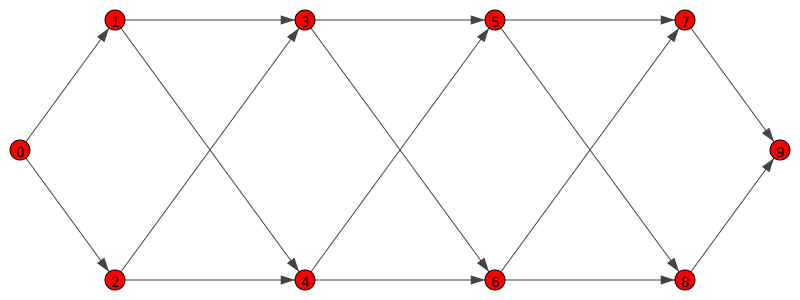
\includegraphics[width=\textwidth]{diamante}
  \caption{In questo esempio di grafo diretto non pesato vediamo che
    esistono esponenziali cammini minimi da $0$ a $9$}
  \label{fig:diamante}
\end{figure}

Vedremo nel capitolo \ref{chap:oracolotutticammini} come salvare
queste informazioni in modo efficiente.

\section{Problema dei $k$ cammini più brevi}

Una generalizzazione del problema dei cammini minimi è il problema dei
$k$ cammini più brevi, cioè dati due vertici $u,v \in V$, ordinati i
cammini in $P(u,v)$ per lunghezza crescente, vogliamo estrarre i primi
$k$ cammini nell'ordine.

In questo caso potremmo dover considerare nuovamente cammini
contenenti cicli, infatti questi (pur non essendo minimi) potrebbero
comparire fra i $k$ cammini più brevi.

Questo problema è molto studiato in letteratura e noi non lo
tratteremo, citeremo solo alcuni risultati.

In \cite{kshortest} vengono forniti algoritmi su grafi diretti per
trovare:
\begin{itemize}
\item dati $u,v \in V$ trovare i primi $k$ cammini più brevi in
  $P\pa{u,v}$ in tempo $O\pa{m + n\log n + k}$
\item una struttura (costruita in $O\pa{m+n\log n}$ tempo) che dati
  $u,v\in V$ ritorna in ordine di lunghezza i cammini in $P(u,v)$
  estraendo l'$i$-esimo in $\log i$ tempo
\item dato $s\in V$ trovare i $k$ cammini più brevi per tutte le
  destinazioni $v\in V$ in $O\pa{m + n\log n + kn}$
\end{itemize}

Uno dei problemi di questi algoritmi è che devono processare tutto il
grafo (che potrebbe essere molto grande) per poter ritornare i primi
$k$ cammini minimi, invece in \cite{kspheur} viene presentato
algoritmo che trova i $k$ cammini più brevi esplorando il grafo
\textit{on-the-fly}, utilizzando delle euristiche per migliorarne le
prestazioni ma ottenendo comunque, al caso pessimo, lo stesso tempo
dell'algoritmo di Eppstein cioè $O\pa{m + n\log n + k}$.

\chapter{Oracoli per distanze}

Ora che sappiamo calcolare la tabella delle distanze ci poniamo il
problema di salvarle. Il metodo banale di farlo (salvare la matrice
delle distanze $D$) richiede $O\pa{ N^2 \log d}$ bit dove $d$ è il
diametro del grafo ($d = O\pa{N}$ nel caso non pesato).

\`E naturale porsi due probelmi:
\begin{itemize}
\item è possibile salvarsi una struttura dati pi\`u piccola ($o
  \pa{ N^2}$) in modo da poter dare ancora una buona approssimazione
  della distanza tra due vertici? Vedremo questo problema nella
  sezione \ref{sec:oracoliapprossimati}
\item qual'\`e la struttura dati pi\`u piccola che contiene le
  informazioni esatte sulle distanza di un grafo? Vedremo questo nella
  sezione \ref{sec:oracoliesatti}
\end{itemize}

\section{Oracoli approssimati}
\label{sec:oracoliapprossimati}

Come gi\`a anticipato, in questa sezione ci poniamo il problema di
usare poco spazio in memoria pur continuando a saper stimare (ma senza
pretendere di restituire il valore esatto) la distanza fra due punti
in un grafo.

Ricordiamo che salvare il grafo completo richiede $O\pa{ N + M } =
O\pa{ N^2}$, per cui dobbiamo cercare degli approci alternativi.

\begin{mydef}[$r$-approssimazione]
  Diciamo che un certo algoritmo ritorna una $r$-approsimazione della
  distanza tra due punti se per ogni $u,v \in V$, detta $d(u,v)$ la
  distanza ritornata dall'algoritmo, si ha che
  \[ d\pa{u,v} \le r \delta\pa{u,v} \]
\end{mydef}

Per questo capitolo useremo grafi non pesati, \`e comunque studiato
anche il caso pesato ma noi lo tralasceremo per semplicit\`a.

\subsection{Graph spanners}

Un metodo molto usato (introdotto in \cite{graphspanners}) consiste
nel salvare (e poi eventualmente preelaborare) un $t$-spanner del
grafo.

\begin{mydef}[$t$-spanner]
  Dato $G = (V,E)$ grafo diciamo che $G' = (V, E')$ \`e un $t$-spanner
  di $G$ se $E' \subseteq E$ e
  \[ \forall u,v \in V \;\; \delta _{G'} \pa{ u,v} \le t \delta _{G}
    \pa{ u,v} \]
  cio\`e la distanza di $G'$ \`e una $t$-approsimazione della distanza
  in $G$.
\end{mydef}

Se quindi troviamo un grafo $G'$ con $o\pa{ N^2}$ archi (per esempio
$O(N)$) con questa propriet\`a allora occupiamo $\tilde O(N \log N)$
spazio per salvarlo e sappiamo rispondere ad una query di distanza in
$O(N)$ (il tempo di eseguire una BFS).

Possiamo caratterizzare un $t$-spanner anche con
\begin{mylem}
  $G' = (V,E')$ con $E' \subseteq E$ \`e un $t$-spanner per $G$ se
  \[ \forall (u,v) \in E\;\; \delta_{G'} (u,v) \le t \]
\end{mylem}
\begin{proof}
  Dalla definizione di $t$ spanner otteniamo facilmente questa
  uguaglianza, per l'implicazione inversa osseriviamo che, dati $u,v
  \in V$, preso un cammino minimo $p \in P(u,v)$ otteniamo la
  disuguaglianza della definizione applicando la disuguaglianza del
  lemma per ogni arco in $p$
\end{proof}

Questo semplice risultato ci mostra che ci sono delle limitazioni
negli spanner che possiamo costruire
\begin{mypro}
  In un grafo indiretto $G = (V,E)$ sia $k$ la lunghezza minima di un
  ciclo non banale in $G$, allora se $G' = (V,E')$ \`e un $t$-spanner
  di $G$ con $t < k-1$ si ha $G = G'$
\end{mypro}
\begin{proof}
  Supponiamo per assurdo che esista $(u,v) \in E' \setminus E$,
  siccome
  \[ \delta_{G'} (u,v) \le t < n -1 \] 

  Si ha che esiste un cammino aciclico composto da $h$ archi di $E'$
  da $u$ a $v$ con $h<k-1$, allora ricordando che $(u,v) \not\in E'$
  si ha che se aggiungiamo $(v,u)$ al cammino otteniamo un ciclo di
  lunghezza $h+1 < k$ da cui l'assuro.
\end{proof}

Ci poniamo allora il problema di dire quando esistono dei $t$-spanner
di un grafo con un certo numero di archi, purtroppo si ha che (teorema
che non dimostriamo)
\begin{myteo}
  Dato un grafo $G = (V,E)$ e due numeri $t,m\ge 1$ il problema di
  determinare se esiste un $t$-spanner di $G$ con al pi\`u $m$ archi
  \`e NP-completo.
\end{myteo}

Nonostante questo teorema \`e possibile studiare il problema in modo
asintotico.

Sempre in \cite{graphspanners} vengono dati i seguenti risultati:

\begin{myteo}
  Dato un grafo di $N$ vertici $G$ e $1<k<N$ esiste (ed \`e
  costruibile in tempo polinomiale) un $(4\log _k N +1)$-spanner con
  al pi\`u $kN$ archi.
\end{myteo}

\begin{mycor}
  Dato un grafo di $N$ vertici $G$ esiste (ed \`e costruibile in tempo
  polinomiale) un $O\pa{\log N}$-spanner con $O(N)$ archi.
\end{mycor}

\begin{mycor}
  Dato un grafo di $N$ vertici $G$ e per ogni $r\ge 1$ esiste (ed \`e
  costruibile in tempo polinomiale) un $(4r+1)$-spanner con
  $O(N^{1+1/r})$ archi.
\end{mycor}


\subsection{Risultati noti}

\section{Oracoli esatti}
\label{sec:oracoliesatti}

Tutte le distanze in $O(n^2)$ spazio con query costanti

http://www.sciencedirect.com/science/article/pii/S0304397510003130

\subsection{Risoluzione tramite alberi di ricoprimento etichettati}

\subsection{Compressione degli alberi}

\subsection{Compressione delle etichette: Wavelet Tree}

\subsection{Ottimalità}

\subsection{Possibile generalizzazione: archi pesati}


\chapter{Oracolo per scrivere tutti i cammini minimi}
\label{chap:oracolotutticammini}

\section{Un primo algoritmo}

$O(n^3)$

\section{Un algoritmo con tempo di query non ottimale}

\subsection{L'algoritmo}

\subsection{Complessità}

\section{Una classe particolare: grafi planari}

\subsection{Separation theorem}

\subsection{Un algoritmo in spazio $O(n^{2.5})$}

$O(n^{2.5})$ con il separation theorem

\section{Un nuovo algoritmo}

???

\section{Un caso difficile}



\bibliographystyle{alpha}
\bibliography{funnymult,apspfmp,kshortest,kspheur,graphspanners}





\end{document}

